% 2005 年山东卷文科第 20 题：长方体直观图与辅助线
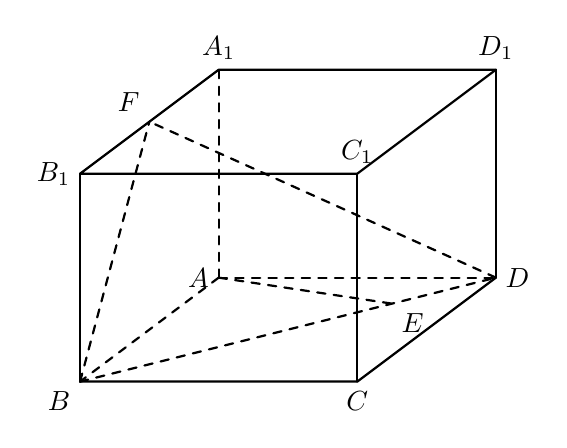
\begin{tikzpicture}[>=stealth,scale=1.1,line cap=round,line join=round]
  % 坐标定义
  % 底面顶点
  \coordinate (A) at (0,0);
  \coordinate (B) at (-1.6,-1.2);
  \coordinate (C) at (1.6,-1.2);
  \coordinate (D) at (3.2,0);

  % 顶面顶点（竖直高度 2.4）
  \coordinate (A1) at (0,2.4);
  \coordinate (B1) at (-1.6,1.2);
  \coordinate (C1) at (1.6,1.2);
  \coordinate (D1) at (3.2,2.4);

  % 中点与垂足
  \coordinate (F) at (-0.8,1.8); % A1B1 中点
  \coordinate (E) at (2.0,-0.3); % AE 垂直 BD 于 E (落在 CC1 右后方)

  % 虚线（不可见棱与辅助线）
  \draw[dashed,thick] (A) -- (A1);
  \draw[dashed,thick] (A) -- (B);
  \draw[dashed,thick] (A) -- (D);
  \draw[dashed,thick] (A) -- (E);
  \draw[dashed,thick] (B) -- (D);
  \draw[dashed,thick] (B) -- (F);
  \draw[dashed,thick] (D) -- (F);

  % 实线（可见棱）
  \draw[thick] (B) -- (C) -- (D);
  \draw[thick] (B) -- (B1);
  \draw[thick] (C) -- (C1);
  \draw[thick] (D) -- (D1);
  \draw[thick] (A1) -- (B1) -- (C1) -- (D1) -- cycle;

  % 顶点标签
  \node[above] at (A1) {$A_1$};
  \node[above] at (D1) {$D_1$};
  \node[left] at (B1) {$B_1$};
  \node[above] at (C1) {$C_1$};
  \node[above left] at (F) {$F$};
  \node[left] at (A) {$A$};
  \node[right] at (D) {$D$};
  \node[below left] at (B) {$B$};
  \node[below] at (C) {$C$};
  \node[below right] at (E) {$E$};
\end{tikzpicture}